\documentclass[11pt,oneside]{article}

\usepackage[a4paper,margin=27mm,headheight=15pt]{geometry}
\usepackage[T1]{fontenc}
\usepackage[utf8]{inputenc}
\IfFileExists{libertinus.sty}{\usepackage{libertinus}}{\usepackage{lmodern}}
\usepackage{microtype}
\usepackage{amsmath,amssymb,amsthm,mathtools}
\usepackage{booktabs,array,tabularx}
\usepackage{graphicx}
\usepackage{pgfplots}
\usepackage{xcolor}
\usepackage{enumitem}
\usepackage{fancyhdr}
\usepackage{titlesec}
\usepackage{xurl}
\usepackage{hyperref}
\usepackage[nameinlink,noabbrev]{cleveref}

\definecolor{linkblue}{RGB}{25,75,135}
\definecolor{shadegray}{RGB}{246,247,249}
\definecolor{rulegray}{RGB}{195,201,208}
\pgfplotsset{compat=1.18}
\hypersetup{
  colorlinks=true,
  linkcolor=linkblue,
  citecolor=linkblue,
  urlcolor=linkblue,
  pdftitle={How Fast Does the Infinite Sinc Product Decay? A Gentle Guide},
  pdfsubject={An accessible companion to the comparative audit of the Rvachev up Fourier decay problem},
  pdfkeywords={sinc product, Fabius function, Rvachev up-function, Fourier decay, Thue-Morse, expository}
}

\pagestyle{fancy}
\fancyhf{}
\fancyhead[L]{\small Gentle guide to the sinc-product decay}
\fancyhead[R]{\small\nouppercase{\leftmark}}
\fancyfoot[C]{\thepage}
\renewcommand{\headrulewidth}{0.4pt}

\titleformat{\section}{\Large\bfseries}{\thesection}{0.7em}{}
\titleformat{\subsection}{\large\bfseries}{\thesubsection}{0.7em}{}
\setcounter{secnumdepth}{2}
\setcounter{tocdepth}{1}
\setlist[itemize]{leftmargin=2em,itemsep=0.25em,topsep=0.4em}
\setlist[enumerate]{leftmargin=2.3em,itemsep=0.25em,topsep=0.4em}
\setlength{\emergencystretch}{2em}

\newtheorem{theorem}{Theorem}[section]
\newtheorem{fact}[theorem]{Fact}
\theoremstyle{remark}
\newtheorem{remark}[theorem]{Remark}

\newcommand{\R}{\mathbb R}
\newcommand{\Z}{\mathbb Z}
\newcommand{\e}{\mathrm e}
\newcommand{\ii}{\mathrm i}
\newcommand{\dd}{\,\mathrm d}
\newcommand{\sinc}{\operatorname{sinc}}
\newcommand{\Up}{\operatorname{up}}

\title{\bfseries How Fast Does the Infinite Sinc Product Decay?\\[0.35em]
\large A gentle guide to the answer, for readers who know limits,
integrals, and a little Fourier analysis}
\author{Companion to the \emph{Comparative Audit} in the same directory\\
\small (which contains the precise statements, proofs, and literature forensics)}
\date{26 August 2026}

\begin{document}
\maketitle

\section*{TL;DR}

\hrule\vspace{0.9em}
\noindent
\textbf{The function.}
$f(x)=\prod_{n=0}^{\infty}\sinc\!\bigl(\pi x/2^n\bigr)$, where
$\sinc z=\frac{\sin z}{z}$.  It is the Fourier transform of the
``smoothest possible bump'': an infinitely differentiable function that
is zero outside $[-1,1]$.  It equals $1$ at $x=0$, vanishes at every
positive integer, and in between it wiggles with rapidly shrinking
humps.

\textbf{How fast it decays.}
Faster than any power of $x$, slower than any exponential.  The precise
shape is
\[
 |f(x)|\;\approx\;
 x^{-\kappa}\cdot
 \exp\!\left(-\frac{(\ln x)^2}{2\ln 2}\right),
\]
where the exponential factor is universal, but---and this is the
punchline---\emph{the power $\kappa$ depends on what you mean by
``how big is $f$ near $x$''}:
\begin{center}
\begin{tabular}{@{}ll@{}}
tallest humps & $\kappa_\infty=2.3590\ldots$\\
mean square (energy) & $\kappa_2=\log_2(2\pi)=2.6515\ldots$\\
plain average of $|f|$ & $\kappa_1=2.7481\ldots$\\
typical point & $\kappa_0=\tfrac32+\log_2\pi=3.1515\ldots$
\end{tabular}
\end{center}
There is no single ``decay rate.''  Asking for one is like asking for
``the income of a country'': the mean, the median, the richest person,
and the root-mean-square are genuinely different numbers.

\textbf{The answer to the Stack Exchange question} (which asks for
$g$ such that the running average of $|f|/g$ tends to $1$): take
\[
 g(x)=0.09127\cdot x^{-2.7481}
 \exp\!\left(-\frac{(\ln x)^2}{2\ln 2}\right).
\]
Then the running average of $|f|/g$ stays between $0.92$ and $1.12$
forever (so the ``bounded'' version of the question is solved), and it
converges to exactly $1$ if you stop the average at powers of two, or
if you average ``per octave'' ($\frac1{\ln t}\int^t\frac{|f|}{g}
\frac{\dd x}{x}$).  But for arbitrary stopping points the limit
provably does \emph{not} exist---for this $g$ or for any other
formula-like $g$.  The average forever oscillates between about
$0.92$ and $1.11$ depending on where between two powers of two you
stop.  That obstruction is a real feature of the function, not a
failure of cleverness.

\textbf{A bonus discovery.}  Cross-checking two of the AI-written
solution drafts against each other exposed a genuine error in a
published 2017 paper (Annales de l'Institut Fourier): a variance was
computed without the factor $\tfrac12$ from
$\int_0^1\cos^2(2\pi kt)\,\dd t=\tfrac12$, making a headline constant
$\sqrt2$ times too large ($\pi$ where it should be $\pi/\sqrt2$).
The five-line correct computation is in \cref{sec:half}.
\par\vspace{0.9em}\hrule

\tableofcontents

\section{The function, and why anyone cares}

Start with the most famous function of signal processing,
\[
 \sinc z=\frac{\sin z}{z},\qquad\sinc 0=1 .
\]
Now multiply infinitely many copies of it, each one stretched twice as
much as the last:
\[
 f(x)=\sinc(\pi x)\cdot\sinc\!\Bigl(\frac{\pi x}{2}\Bigr)\cdot
 \sinc\!\Bigl(\frac{\pi x}{4}\Bigr)\cdot
 \sinc\!\Bigl(\frac{\pi x}{8}\Bigr)\cdots
\]
The product converges nicely: for large $n$ the factor
$\sinc(\pi x/2^n)$ is extremely close to $1$ (since $\sinc z\approx
1-z^2/6$ near $0$), so past some point the factors stop mattering.

Why this particular product?  Because $\sinc$ is the Fourier transform
of a rectangular pulse, and multiplying Fourier transforms means
\emph{convolving} the originals.  So $f$ is the Fourier transform of
the infinite convolution of rectangles of widths $1,\tfrac12,\tfrac14,
\dots$ --- a famous function called $\Up(t)$ (Rvachev's
\emph{up-function}, a close relative of the Fabius function): a
perfectly smooth bump, infinitely differentiable, exactly zero outside
$[-1,1]$.  Smooth compactly supported functions have rapidly decaying
Fourier transforms, so $f$ must die faster than any power of $x$.  The
question --- asked on Mathematics Stack Exchange in 2018 and the subject
of this directory --- is: \emph{exactly how fast?}

Three visible features of $f$, all easy to believe and all proved in
the audit:
\begin{itemize}
\item $f(m)=0$ for every nonzero integer $m$ (already the first factor
$\sinc(\pi x)$ vanishes there);
\item between consecutive integers, $|f|$ makes exactly one hump;
\item the \emph{sign} of $f$ on the interval $(m,m+1)$ is
$(-1)^{(\text{number of 1's in the binary digits of }m)}$ --- the
Thue--Morse pattern:
\begin{center}
\begin{tabular}{@{}l*{8}{c}@{}}
\toprule
$m$ & 0 & 1 & 2 & 3 & 4 & 5 & 6 & 7\\
binary & 0 & 1 & 10 & 11 & 100 & 101 & 110 & 111\\
sign of $f$ on $(m,m+1)$ & $+$ & $-$ & $-$ & $+$ & $-$ & $+$ & $+$ & $-$\\
\bottomrule
\end{tabular}
\end{center}
Binary digits will keep showing up.  That is not a coincidence: the
factor scales are powers of $2$, so everything about this function is
secretly about binary expansions.
\end{itemize}

\section{How small is it, really?}

Some honest numbers, computed directly from the product:
\[
 |f(10.5)|\approx10^{-5.0},\qquad
 |f(100.5)|\approx10^{-13.0},\qquad
 |f(1000.5)|\approx10^{-26.4}.
\]
Each factor-of-ten step in $x$ roughly \emph{doubles} the number of
zeros after the decimal point, rather than adding a fixed number.
That is the signature of a law like
$\exp(-c(\ln x)^2)$: the exponent is \emph{quadratic} in $\ln x$.  A
plain power law $x^{-p}$ would add the same $p$ digits per decade;
an exponential $\e^{-cx}$ would multiply the digits by ten per decade.
This function sits exactly in between, and the questioner's original
guess, ``something close to $\exp(-\ln^2x)$,'' was pointing at the
right family.  The correct constant turns out to be
$\frac{1}{2\ln2}=0.7213\ldots$ in place of $1$, and on top of the
$\exp(-(\ln x)^2/(2\ln2))$ factor there is a power of $x$ that carries
all the interesting mathematics.  Let us see where each part comes
from.

\section{Where the \texorpdfstring{$\exp(-(\ln x)^2/(2\ln2))$}{exp(-ln²x/2ln2)} comes from: just count}

Fix a large $x$, say $x=1000$, and look at the factors
$\sinc(\pi x/2^n)$ one at a time.

\begin{itemize}
\item If $2^n$ is \emph{much bigger} than $x$, the argument
$\pi x/2^n$ is tiny and the factor is essentially $1$.  Harmless.
\item If $2^n$ is \emph{smaller} than $x$ (for $x=1000$ that means
$n=0,1,\dots,9$, since $2^9=512<1000<1024=2^{10}$), the argument is
large, and
\[
 \Bigl|\sinc\!\Bigl(\frac{\pi x}{2^n}\Bigr)\Bigr|
 =\frac{|\sin(\pi x/2^n)|}{\pi x/2^n}
 \le\frac{2^n}{\pi x}.
\]
Each of these factors is \emph{small}, and there are about
$k+1\approx\log_2x$ of them.
\end{itemize}
Multiply the small ones together, ignoring the sines for a moment:
\[
 \prod_{n=0}^{k}\frac{2^n}{\pi x}
 =\frac{2^{0+1+\cdots+k}}{(\pi x)^{k+1}}
 =\frac{2^{k(k+1)/2}}{(\pi x)^{k+1}},
 \qquad k\approx\log_2 x .
\]
Now take logarithms and keep the biggest term.  With
$k\approx\ln x/\ln2$,
\[
 \ln\Bigl(\text{product}\Bigr)
 \approx\frac{k^2}{2}\ln 2-k\ln(\pi x)
 \approx\frac{(\ln x)^2}{2\ln2}-\frac{(\ln x)^2}{\ln 2}
 =-\frac{(\ln x)^2}{2\ln 2}.
\]
That is the whole story of the universal factor: \emph{about
$\log_2x$ factors, each of size roughly $2^n/x$}.  For $x=1000$ this
crude count predicts $|f|\lesssim10^{-21.4}$; the actual typical size
$10^{-26}$ is smaller because we threw away the sine factors, which
brings us to the interesting part.

\section{The wild part: sines and binary digits}

The neglected numerators are
\[
 \bigl|\sin(\pi x)\bigr|\cdot
 \bigl|\sin(\pi x/2)\bigr|\cdots
 \bigl|\sin(\pi x/2^k)\bigr| ,
\]
a product of about $\log_2x$ numbers, each between $0$ and $1$.  How
big is such a product?  Here is the key trick.  Since
$|\sin(\pi t)|$ only depends on $t$ modulo $1$, only the
\emph{fractional parts} of $x,\ x/2,\ x/4,\dots$ matter.  And halving
a number shifts its binary digits: if
\[
 x=1101101.0110101\ldots\ \text{(binary)},
\]
then $x/2=110110.10110101\ldots$, $x/4=11011.010110101\ldots$, and so
on.  Each factor $|\sin(\pi x/2^n)|$ reads the binary expansion of $x$
\emph{through a window shifted by $n$ places}.  A product over $n$ of
such factors is therefore a walk along the binary digits of $x$ ---
and binary digits of a typical number behave like coin flips.  Two
consequences:

\begin{itemize}
\item \emph{On average, each sine factor costs a factor
$\tfrac12$.}  The average of $\ln|\sin(\pi t)|$ over $t\in[0,1]$ is
$-\ln2$ (a classical integral).  So a typical product of $k$ sines is
about $2^{-k}$, which for $x=1000$ ($k\approx10$) accounts for
the missing $10^{-3}$ between the crude bound $10^{-21.4}$ and reality
$\approx10^{-26}$ --- well, most of it; the rest is bookkeeping in the
crude estimate itself.
\item \emph{But the fluctuations around ``typical'' are enormous.}
The factors are like random numbers, and a product of $k$ random
factors has a spread that grows with $k$: the logarithm performs a
random-walk-like motion of typical size $\sqrt{k}$ around its mean
(with variance $\pi^2/4$ per step --- this specific constant is the
star of \cref{sec:half}).  Since multiplying by $\e^{\pm c\sqrt{k}}$
means gaining or losing several \emph{orders of magnitude}, nearby
values of $x$ can give wildly different $|f(x)|$.
\end{itemize}

There is one special binary pattern worth knowing.  If the fractional
part of $x$ is $\tfrac13=0.010101\ldots$ (binary), then shifting the
digits alternates between $0.0101\ldots=\tfrac13$ and
$0.1010\ldots=\tfrac23$, and every sine factor equals
$\sin(\pi/3)=\tfrac{\sqrt3}{2}=0.866$ --- the largest sustainable
value.  No point can keep \emph{all} its sine factors near $1$:
if $t$ is close to $\tfrac12$ (where $\sin(\pi t)=1$), then $2t$ is
close to $0$ or $1$ (where the sine \emph{vanishes}).  Staying on the
$\tfrac13\leftrightarrow\tfrac23$ cycle is the best compromise, and
this single fact (the ``Gelfond bound,'' proved in the audit by a
two-line algebraic inequality) pins down the tallest humps of $f$.

\section{One octave under the microscope}

Everything above becomes visible if we plot, for every unit interval
$[n,n+1]$ inside one ``octave'' $[512,1024]$, the height $E_n$ of the
single hump of $|f|$ there.

\begin{figure}[ht]
\centering
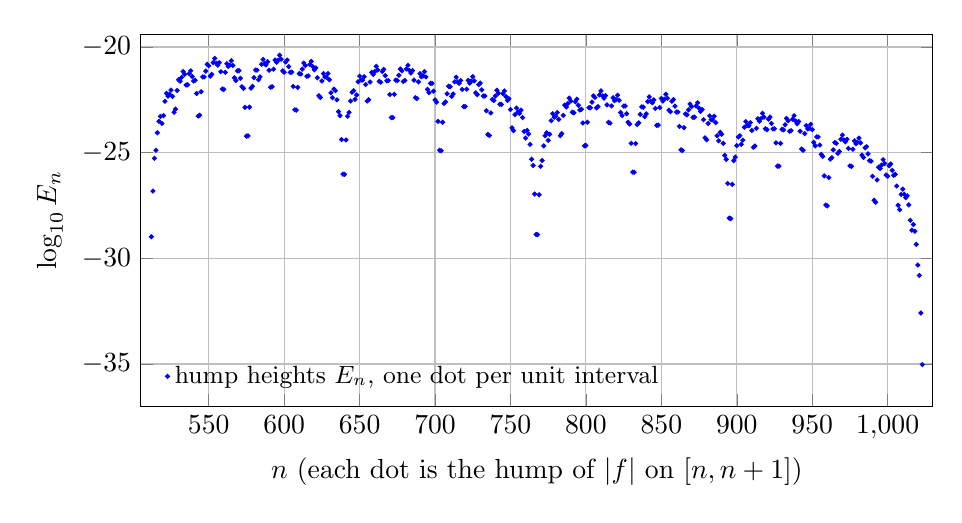
\begin{tikzpicture}
\begin{axis}[
 width=0.96\textwidth, height=0.52\textwidth,
 xlabel={$n$ (each dot is the hump of $|f|$ on $[n,n+1]$)},
 ylabel={$\log_{10}E_n$},
 xmin=505, xmax=1030, ymin=-37, ymax=-19.4,
 grid=major,
 legend style={at={(0.02,0.02)},anchor=south west,draw=none,fill=none,
   font=\small},
]
\addplot+[only marks, mark size=0.7pt] coordinates {
(512,-28.98) (513,-26.82) (514,-25.27) (515,-24.89) (516,-24.06) (517,-23.52) (518,-23.29) (519,-23.62) (520,-23.25) (521,-22.57) (522,-22.20) (523,-22.33) (524,-22.24) (525,-22.04) (526,-22.34) (527,-23.09) (528,-22.94) (529,-22.06) (530,-21.55) (531,-21.62) (532,-21.44) (533,-21.16) (534,-21.29) (535,-21.80) (536,-21.79) (537,-21.26) (538,-21.13) (539,-21.40) (540,-21.61) (541,-21.57) (542,-22.20) (543,-23.27) (544,-23.23) (545,-22.12) (546,-21.42) (547,-21.42) (548,-21.14) (549,-20.82) (550,-20.89) (551,-21.38) (552,-21.30) (553,-20.74) (554,-20.54) (555,-20.77) (556,-20.86) (557,-20.74) (558,-21.17) (559,-21.99) (560,-22.01) (561,-21.20) (562,-20.79) (563,-20.92) (564,-20.86) (565,-20.65) (566,-20.88) (567,-21.46) (568,-21.59) (569,-21.13) (570,-21.12) (571,-21.48) (572,-21.88) (573,-21.96) (574,-22.86) (575,-24.22) (576,-24.21) (577,-22.85) (578,-21.95) (579,-21.86) (580,-21.45) (581,-21.09) (582,-21.10) (583,-21.55) (584,-21.41) (585,-20.82) (586,-20.59) (587,-20.79) (588,-20.85) (589,-20.70) (590,-21.10) (591,-21.91) (592,-21.88) (593,-21.05) (594,-20.62) (595,-20.73) (596,-20.63) (597,-20.39) (598,-20.58) (599,-21.13) (600,-21.20) (601,-20.71) (602,-20.62) (603,-20.93) (604,-21.20) (605,-21.19) (606,-21.87) (607,-22.97) (608,-22.99) (609,-21.91) (610,-21.26) (611,-21.28) (612,-21.05) (613,-20.76) (614,-20.88) (615,-21.39) (616,-21.37) (617,-20.83) (618,-20.68) (619,-20.93) (620,-21.08) (621,-20.99) (622,-21.46) (623,-22.31) (624,-22.39) (625,-21.61) (626,-21.26) (627,-21.42) (628,-21.43) (629,-21.26) (630,-21.55) (631,-22.17) (632,-22.40) (633,-21.99) (634,-22.07) (635,-22.50) (636,-23.06) (637,-23.25) (638,-24.38) (639,-26.02) (640,-26.03) (641,-24.40) (642,-23.28) (643,-23.10) (644,-22.56) (645,-22.14) (646,-22.07) (647,-22.48) (648,-22.27) (649,-21.65) (650,-21.38) (651,-21.56) (652,-21.57) (653,-21.41) (654,-21.78) (655,-22.56) (656,-22.50) (657,-21.66) (658,-21.20) (659,-21.30) (660,-21.17) (661,-20.92) (662,-21.09) (663,-21.63) (664,-21.67) (665,-21.16) (666,-21.06) (667,-21.36) (668,-21.60) (669,-21.59) (670,-22.25) (671,-23.34) (672,-23.34) (673,-22.24) (674,-21.57) (675,-21.59) (676,-21.34) (677,-21.04) (678,-21.13) (679,-21.63) (680,-21.59) (681,-21.04) (682,-20.87) (683,-21.11) (684,-21.23) (685,-21.12) (686,-21.57) (687,-22.40) (688,-22.44) (689,-21.65) (690,-21.26) (691,-21.41) (692,-21.37) (693,-21.17) (694,-21.42) (695,-22.01) (696,-22.16) (697,-21.72) (698,-21.72) (699,-22.09) (700,-22.51) (701,-22.61) (702,-23.52) (703,-24.89) (704,-24.91) (705,-23.56) (706,-22.67) (707,-22.60) (708,-22.21) (709,-21.86) (710,-21.88) (711,-22.34) (712,-22.22) (713,-21.65) (714,-21.43) (715,-21.65) (716,-21.72) (717,-21.59) (718,-22.01) (719,-22.82) (720,-22.82) (721,-22.00) (722,-21.58) (723,-21.71) (724,-21.62) (725,-21.40) (726,-21.61) (727,-22.17) (728,-22.26) (729,-21.78) (730,-21.71) (731,-22.03) (732,-22.32) (733,-22.32) (734,-23.02) (735,-24.14) (736,-24.19) (737,-23.12) (738,-22.49) (739,-22.53) (740,-22.32) (741,-22.05) (742,-22.19) (743,-22.71) (744,-22.72) (745,-22.21) (746,-22.08) (747,-22.35) (748,-22.53) (749,-22.45) (750,-22.96) (751,-23.83) (752,-23.96) (753,-23.20) (754,-22.89) (755,-23.08) (756,-23.14) (757,-22.99) (758,-23.34) (759,-24.00) (760,-24.31) (761,-23.95) (762,-24.12) (763,-24.61) (764,-25.31) (765,-25.61) (766,-26.96) (767,-28.87) (768,-28.88) (769,-26.99) (770,-25.65) (771,-25.37) (772,-24.68) (773,-24.20) (774,-24.06) (775,-24.42) (776,-24.13) (777,-23.49) (778,-23.16) (779,-23.32) (780,-23.28) (781,-23.10) (782,-23.43) (783,-24.20) (784,-24.10) (785,-23.24) (786,-22.75) (787,-22.84) (788,-22.68) (789,-22.42) (790,-22.56) (791,-23.09) (792,-23.11) (793,-22.59) (794,-22.47) (795,-22.76) (796,-22.98) (797,-22.95) (798,-23.60) (799,-24.68) (800,-24.66) (801,-23.56) (802,-22.87) (803,-22.88) (804,-22.61) (805,-22.31) (806,-22.39) (807,-22.88) (808,-22.82) (809,-22.27) (810,-22.08) (811,-22.31) (812,-22.42) (813,-22.30) (814,-22.74) (815,-23.57) (816,-23.60) (817,-22.79) (818,-22.40) (819,-22.54) (820,-22.49) (821,-22.28) (822,-22.52) (823,-23.10) (824,-23.25) (825,-22.80) (826,-22.79) (827,-23.16) (828,-23.56) (829,-23.65) (830,-24.56) (831,-25.92) (832,-25.93) (833,-24.57) (834,-23.67) (835,-23.59) (836,-23.19) (837,-22.83) (838,-22.85) (839,-23.30) (840,-23.17) (841,-22.59) (842,-22.36) (843,-22.57) (844,-22.64) (845,-22.50) (846,-22.91) (847,-23.71) (848,-23.70) (849,-22.87) (850,-22.44) (851,-22.56) (852,-22.47) (853,-22.24) (854,-22.43) (855,-22.99) (856,-23.06) (857,-22.57) (858,-22.49) (859,-22.80) (860,-23.08) (861,-23.08) (862,-23.76) (863,-24.87) (864,-24.90) (865,-23.82) (866,-23.17) (867,-23.21) (868,-22.98) (869,-22.70) (870,-22.82) (871,-23.33) (872,-23.32) (873,-22.79) (874,-22.64) (875,-22.90) (876,-23.05) (877,-22.96) (878,-23.44) (879,-24.30) (880,-24.39) (881,-23.62) (882,-23.26) (883,-23.44) (884,-23.45) (885,-23.28) (886,-23.58) (887,-24.20) (888,-24.44) (889,-24.04) (890,-24.13) (891,-24.56) (892,-25.13) (893,-25.32) (894,-26.46) (895,-28.10) (896,-28.12) (897,-26.50) (898,-25.38) (899,-25.21) (900,-24.67) (901,-24.26) (902,-24.20) (903,-24.61) (904,-24.41) (905,-23.80) (906,-23.53) (907,-23.71) (908,-23.73) (909,-23.58) (910,-23.95) (911,-24.75) (912,-24.69) (913,-23.85) (914,-23.40) (915,-23.51) (916,-23.39) (917,-23.14) (918,-23.32) (919,-23.87) (920,-23.91) (921,-23.42) (922,-23.32) (923,-23.62) (924,-23.88) (925,-23.87) (926,-24.54) (927,-25.64) (928,-25.64) (929,-24.56) (930,-23.90) (931,-23.92) (932,-23.68) (933,-23.38) (934,-23.49) (935,-23.99) (936,-23.96) (937,-23.42) (938,-23.25) (939,-23.50) (940,-23.63) (941,-23.53) (942,-23.99) (943,-24.83) (944,-24.89) (945,-24.10) (946,-23.72) (947,-23.88) (948,-23.85) (949,-23.66) (950,-23.91) (951,-24.51) (952,-24.68) (953,-24.25) (954,-24.26) (955,-24.64) (956,-25.08) (957,-25.18) (958,-26.10) (959,-27.48) (960,-27.52) (961,-26.18) (962,-25.31) (963,-25.24) (964,-24.87) (965,-24.52) (966,-24.56) (967,-25.03) (968,-24.94) (969,-24.37) (970,-24.17) (971,-24.40) (972,-24.49) (973,-24.37) (974,-24.80) (975,-25.63) (976,-25.65) (977,-24.84) (978,-24.44) (979,-24.58) (980,-24.52) (981,-24.31) (982,-24.54) (983,-25.12) (984,-25.23) (985,-24.77) (986,-24.72) (987,-25.06) (988,-25.38) (989,-25.40) (990,-26.12) (991,-27.25) (992,-27.35) (993,-26.29) (994,-25.69) (995,-25.75) (996,-25.59) (997,-25.33) (998,-25.51) (999,-26.06) (1000,-26.12) (1001,-25.62) (1002,-25.54) (1003,-25.84) (1004,-26.07) (1005,-26.03) (1006,-26.58) (1007,-27.49) (1008,-27.70) (1009,-26.98) (1010,-26.73) (1011,-26.97) (1012,-27.13) (1013,-27.04) (1014,-27.47) (1015,-28.20) (1016,-28.67) (1017,-28.40) (1018,-28.72) (1019,-29.34) (1020,-30.32) (1021,-30.81) (1022,-32.59) (1023,-35.03)
};
\addlegendentry{hump heights $E_n$, one dot per unit interval}
\end{axis}
\end{tikzpicture}
\caption{All $512$ hump heights of $|f|$ in the octave
$[512,1024]$, on a $\log_{10}$ scale.  Note the range: from
$10^{-20.4}$ (near $n=597$) down to $10^{-35}$ (the last hump before
$1024$) --- \emph{fifteen orders of magnitude inside a single
octave}.  The downward spikes sit at $640=5\cdot2^7$,
$768=3\cdot2^8$, $896=7\cdot2^7$, \dots: the more factors of $2$ in
$n$, the deeper the dip.  The tallest hump sits near
$512\cdot\tfrac76\approx597$, whose fractional dynamics locks onto the
optimal $\tfrac13\leftrightarrow\tfrac23$ binary cycle.}
\label{fig:octave}
\end{figure}

Three lessons from \cref{fig:octave}:

\begin{enumerate}
\item \textbf{The dips are at multiples of powers of two.}  Why?  At
$x=2^j\cdot(\text{odd})$, not just one factor but $j+1$ factors of the
product vanish simultaneously: $\sin(\pi x)$, $\sin(\pi x/2)$,
\dots, $\sin(\pi x/2^{j})$ all hit an integer argument.  A zero of
multiplicity $j+1$ crushes its neighborhood, so the humps next to
``very even'' integers are exceptionally tiny.  The extreme case is
the hump just before $1024=2^{10}$: height $10^{-35}$, against
$10^{-20.4}$ for the best hump of the same octave.
\item \textbf{The tallest humps live near mantissa $7/6$.}
$597/512\approx7/6$, and $\tfrac76-1=\tfrac16$ reaches the optimal
cycle $\tfrac13$ after one digit shift.  (As $x$ grows, the best
mantissa slowly drifts toward $1$; the audit computes this drift
exactly, with a Lambert-$W$ function.)
\item \textbf{``The'' size of $f$ near $x=700$ is not one number.}
Within this single octave, the tallest hump, the average hump, the
root-mean-square hump, and the median hump are already visibly
different scales --- and the gaps between them \emph{grow} as a power
of $x$.  That is the content of the next section.
\end{enumerate}

\section{Four legitimate answers to ``how fast does it decay?''}
\label{sec:four}

Think of the humps in an octave as incomes in a country: a few
enormous ones, a broad middle class, and a long tail of tiny ones
(spread over many orders of magnitude --- roughly ``log-normal,'' like
real incomes).  Then:

\begin{center}
\begin{tabularx}{\textwidth}{@{}lllX@{}}
\toprule
question & analogy & answer & value of $\kappa$\\
\midrule
biggest value near $x$? & richest person &
$x^{-\kappa_\infty}\exp\bigl(-\tfrac{(\ln x)^2}{2\ln2}\bigr)$ &
$\kappa_\infty=\tfrac32+\log_2\tfrac{\pi}{\sqrt3}=2.3590$\\[0.3em]
root-mean-square? & RMS income &
same shape & $\kappa_2=\log_2(2\pi)=2.6515$\\[0.3em]
plain average of $|f|$? & mean income &
same shape & $\kappa_1=\tfrac12+\log_2\tfrac{\pi}{\varrho}=2.7481$\\[0.3em]
typical value? & median income &
same shape & $\kappa_0=\tfrac32+\log_2\pi=3.1515$\\
\bottomrule
\end{tabularx}
\end{center}

All four share the universal factor
$\exp(-(\ln x)^2/(2\ln2))$ from the counting argument; they differ in
the power of $x$, because they weigh the huge-but-rare humps
differently.  ``Biggest'' is dominated by the $\tfrac13$-cycle
(that is where $\sqrt3$ enters).  ``Root-mean-square'' turns out to be
\emph{exactly} computable (\cref{sec:rms}) --- that is where the neat
closed form $\log_2(2\pi)$ comes from, and it is precisely the
exponent that an old draft in this repository proposed, mistaking it
for a pointwise decay rate.  ``Average'' involves a constant
$\varrho=0.661322602\ldots$ with no known closed form: it is the
growth rate of the integrals
$\int_0^1|\sin(\pi t)\sin(2\pi t)\cdots\sin(2^{k-1}\pi t)|\,\dd t
\approx\text{const}\cdot\varrho^{\,k}$, a number studied in analytic
number theory (Fouvry--Mauduit).  ``Typical'' comes from the
average-cost-$\tfrac12$-per-factor rule.

Note the moral: if you simulate the function and eyeball a slope, the
answer you get depends entirely on \emph{what you averaged before
taking the slope}.  Several plausible-looking published and drafted
formulas for ``the'' decay rate of this function differ exactly
because each implicitly chose a different row of this table.

\section{The answer to the Stack Exchange question}
\label{sec:answer}

The original question asks for a nice function $g$ (positive, smooth,
decreasing) such that
\[
 \frac{1}{t-t_0}\int_{t_0}^{t}\frac{|f(x)|}{g(x)}\,\dd x
 \;\longrightarrow\;1
 \qquad\text{as } t\to\infty .
 \tag{$\ast$}
\]
Averaging $|f|/g$ is asking $g$ to be the \emph{mean} size of $|f|$
--- so, by the table, $g$ must be the $\kappa_1$ row.  The audited
answer:
\[
 \boxed{\;
 g(x)=A_1\,x^{-\kappa_1}
 \exp\!\left(-\frac{(\ln x)^2}{2\ln 2}\right),
 \qquad
 \kappa_1=2.748070\ldots,\quad
 A_1=0.0912661\ldots
 \;}
\]
And then:

\begin{itemize}
\item \textbf{The bounded version of the question is fully solved.}
The running average of $|f|/g$ stays between $0.92$ and $1.12$ for all
large $t$.  (The question offered this as an acceptable fallback ---
condition (3) in the original post.)
\item \textbf{The limit ($\ast$) holds along $t=1,2,4,8,\dots$}: if
you always stop the average at a power of two, it converges to
exactly $1$ (numerically it is $1.000000$ from $t=2^9$ on).
\item \textbf{But for arbitrary $t$ the limit provably fails} ---
for this $g$ and for every $g$ given by any formula of the usual
kind.  Instead, the average approaches a periodic-in-$\log_2t$
profile: stopping at $t=1.15\cdot2^k$ always gives about $0.92$,
stopping at $t=1.43\cdot2^k$ always gives about $1.11$.
\end{itemize}

Why can no clever $g$ fix this?  Two ingredients.

\emph{First ingredient: the last octave never fades.}  In a running
average up to $t$, the chunk between $t/2$ and $t$ occupies half the
interval --- always.  So the average never stops caring about the most
recent octave, and if the mass of $|f|$ is distributed unevenly
\emph{inside} each octave in a way that repeats from octave to octave,
the average inherits that unevenness forever.  (Contrast a function
whose ``pattern length'' stays fixed while $t\to\infty$: then any one
pattern eventually occupies a vanishing fraction of $[0,t]$ and
averages out.  Here the pattern is multiplicative --- it doubles with
$t$ --- so it never dilutes.)

\emph{Second ingredient: inside one octave, the mass distribution is
fractal.}  One might hope to build the octave profile into $g$.  The
obstruction: as $k\to\infty$ the fraction of the octave-mass of
$|f|$ lying in the first $100\theta\%$ of the octave converges to a
function $F(\theta)$ that is continuous but \emph{singular} --- it
rises, like the devil's staircase, on a set that a smooth density
cannot see (most of the rise happens near mantissas related to the
$\tfrac13$-cycle).  A smooth $g$ can only reweight the octave by a
smooth factor, and no smooth reweighting turns a staircase into a
straight line.  That is the rigorous content of ``the histogram never
flattens,'' and it is proved in the audit with a pleasantly low-tech
argument (if the limiting distribution had a density, iterating the
digit-shift would blow the density up beyond any integrable bound).

\emph{The repair.}  The mismatch is between an \emph{additive} average
($\dd x$, which overweights the last octave) and a
\emph{multiplicative} function (whose natural period is the octave).
Average multiplicatively instead --- give every octave equal weight:
\[
 \frac{1}{\ln(t/t_0)}\int_{t_0}^{t}\frac{|f(x)|}{g(x)}\,
 \frac{\dd x}{x}
 \;\longrightarrow\;\text{const}
 \qquad\text{for \emph{all} } t\to\infty,
\]
because now the final partial octave carries weight
$\sim1/\ln t\to0$.  With the constant absorbed into $g$, the exact
analogue of ($\ast$) holds with no restriction on $t$.  In one
sentence: \emph{the question as posed has answer ``no, but'': no for
the literal limit, yes for the bounded version, yes along powers of
two, and yes for every $t$ once the average respects the function's
own dyadic geometry.}

\section{The missing \texorpdfstring{$\tfrac12$}{1/2}: a cautionary tale}
\label{sec:half}

While cross-checking the four AI-written solutions, two of them
disagreed about a fluctuation constant: one derived
$\pi/\sqrt2$, the other quoted $\pi$ from a 2017 paper in the
\emph{Annales de l'Institut Fourier}.  Both could not be right, and
the disagreement is settled by a computation short enough to do here.
The quantity is the variance of
\[
 S_k(t)=\sum_{j=0}^{k-1}\ln\bigl|2\sin(\pi 2^jt)\bigr| ,
\]
with $t$ drawn uniformly from $[0,1]$ (this is exactly the logarithm
of the sine product from \cref{sec:four}, with the convenient
$2$'s making each term average to zero).  Three steps:

\begin{enumerate}
\item \emph{Fourier series.}  Classically,
$\ln|2\sin\pi t|=-\sum_{m\ge1}\frac{\cos(2\pi mt)}{m}$.
\item \emph{Variance of one term.}  By Parseval --- remembering
$\int_0^1\cos^2(2\pi mt)\,\dd t=\tfrac12$ ---
\[
 \int_0^1\ln^2|2\sin\pi t|\,\dd t
 =\frac12\sum_{m\ge1}\frac1{m^2}
 =\frac{\pi^2}{12}.
\]
\item \emph{Correlations between terms.}  Term $j$ and term $j+r$
share only the frequencies where $m=2^r m'$, giving
\[
 \int_0^1\ln|2\sin\pi t|\cdot\ln|2\sin(\pi 2^rt)|\,\dd t
 =\frac12\sum_{m'\ge1}\frac{1}{2^rm'^2}\cdot\frac1{m'}\cdot m'
 =\frac{\pi^2}{12}\cdot\frac{1}{2^r},
\]
and summing the whole covariance array,
\[
 \frac{\operatorname{Var}S_k}{k}\longrightarrow
 \frac{\pi^2}{12}\Bigl(1+2\sum_{r\ge1}2^{-r}\Bigr)
 =\frac{\pi^2}{12}\cdot3
 =\frac{\pi^2}{4}.
\]
\end{enumerate}
So the ``standard deviation per factor'' is $\pi/2$, and the standard
theory of such sums then gives fluctuation constants proportional to
$\sqrt{\pi^2/4}$ --- producing the $\pi/\sqrt2$ of the first document.
The published paper's equation (4.5) evaluates \emph{the same
variance} but with each Parseval $\tfrac12$ replaced by $1$, obtaining
$\pi^2/2$ and hence constants $\sqrt2$ too large.  The slip is
verified three ways in the audit: against the publisher's PDF, against
the authors' own \LaTeX{} source, and --- most convincingly --- by
simulating $S_{1000}$ on four million exactly-computed binary orbits:
measured variance $2459.5$, against $2464.1$ predicted by
$\pi^2/4$ and $4928.2$ predicted by $\pi^2/2$.  Verdict: the paper's
Theorems 1.1 and 1.2 hold with their constants divided by $\sqrt2$.
(The repository now carries, next to the transcription of the original,
a corrected edition of the whole paper ---
\nolinkurl{AIF_2017__67_2_637_0-corrected.tex} under
\nolinkurl{docs/papers/} --- whose constants match this computation.)

Two morals for the working mathematician.  First,
$\int\cos^2=\tfrac12$ has claimed another victim; check your
Parsevals.  Second, the error was found \emph{not} by checking a
document against the literature --- the second document matched the
literature perfectly --- but by insisting that two independent
derivations agree with each other, and then measuring the disputed
quantity.  Faithful citation is not correctness.

\section{The humps, and the mean-square miracle}
\label{sec:rms}

Two more findings from the expanded audit, in friendly form.

\textbf{Hump heights are glued to areas.}  Each hump is a smooth arch,
so its height and its area (the integral of $|f|$ over the unit
interval) should be comparable --- and they are, provably within a
factor $C(\ln n)^3$ and in practice much tighter: across whole
octaves,
\[
 \frac{\text{sum of hump heights}}{\text{integral of }|f|}
 =1.9237\ldots,
\]
constant to five digits from $x=512$ to $x=32768$.  Consequently the
\emph{average hump height} obeys the same $\kappa_1$ law as the
average of $|f|$ --- the ``envelope of maxima'' reading of the
question and the ``running mean'' reading collapse into one, which is
reassuring.  (The typical hump, by contrast, follows the
$\kappa_0$ law, and the histogram of $\log$-heights within an octave
approaches a bell curve of width $\tfrac\pi2\sqrt{\log_2x}$, visibly
clipped on the right by the $\tfrac13$-cycle ceiling --- all of this
is quantified in the audit.)

\textbf{Squares are where God smiles.}  Replace $|f|$ by $f^2$
(energy, in signal-processing terms) and everything becomes exact,
essentially because $\sin^2$ has the clean average $\tfrac12$ and
because of binary uniqueness.  A sample, provable in a few lines
each:
\[
 \int_0^1\prod_{j=0}^{k-1}\sin^2(\pi2^jt)\,\dd t=\frac{1}{2^k}
 \quad\text{exactly, for every }k,
\]
(write each $\sin^2$ as $\tfrac12(1-\cos)$; expanding the product
gives cosines whose frequencies are sums of \emph{distinct} powers of
two, and by uniqueness of binary representation none of them can
cancel to frequency zero, so only the constant term survives);
and the total energy identity
\[
 \int_{-\infty}^{\infty}f(x)^2\dd x
 =\int_{-1}^{1}\Up(t)^2\dd t
 =\frac12+\sum_{m=0}^{\infty}f\Bigl(m+\tfrac12\Bigr)^{2}
 =0.8088735359679\ldots,
\]
which is just Parseval's theorem for the Fourier series of the bump
$\Up$ on $[-1,1]$ (its Fourier coefficients are values of $f$ at
half-integers!).  The two sides were computed independently and agree
to $2\cdot10^{-15}$ --- a pleasant end-to-end check that every formula
in this story is what it claims to be.  The mean-square envelope even
converges at a knowable geometric rate: the relevant averaging
operator has second eigenvalue exactly $-\tfrac14$ (eigenfunctions
$\sin2\pi x$ and $1+3\cos2\pi x$ --- a two-line verification), so the
RMS constant settles with error $\sim(-\tfrac12)^k$ per octave,
alternating in sign, precisely as the measurements show.

One last warning flows from the same circle of ideas.  Since
$\ln|f|$ fluctuates like a random walk, it is tempting to model
$|f|$ as log-normal and predict the mean and mean-square from the
bell curve.  This fails badly --- the bell-curve model predicts
$\kappa_2\approx-0.41$ (i.e.\ moment \emph{growth}) against the true
$2.65$ --- because the extreme humps that would dominate such averages
are capped by the $\tfrac13$-cycle ceiling.  The correct
moment-generating object is the $\kappa_q$ curve itself, which is
exactly what the four-row table of \cref{sec:four} samples.

\section{What to remember}

\begin{enumerate}
\item $f$ decays like
$x^{-\kappa}\exp\bigl(-(\ln x)^2/(2\ln2)\bigr)$: the exponential
factor comes from \emph{counting factors}, and is universal.
\item The power $\kappa$ is not unique: biggest/mean-square/mean/typical
give $2.359<2.651<2.748<3.151$.  Any claim about ``the'' decay rate
must say which average it means.
\item The literal limit requested on Stack Exchange is unattainable
(last-octave effect + fractal octave profile), but the bounded
version, the powers-of-two version, and the per-octave version are
all solved by
$g=0.0913\,x^{-2.748}\exp(-(\ln x)^2/(2\ln2))$.
\item Binary digits run the show: signs are Thue--Morse, valleys sit
at multiples of powers of two, peaks lock onto the binary cycle of
$\tfrac13$, and the constant $\varrho=0.6613\ldots$ is a genuinely new
number of this dyadic world.
\item $\int_0^1\cos^2=\tfrac12$.  Even the Annales de l'Institut
Fourier forgot it once.
\end{enumerate}

\section{Where to find the real proofs}

Everything asserted here is stated precisely and proved (or explicitly
labeled as imported/conjectural) in the companion document
\emph{The Decay Envelope of the Rvachev Sinc Product: A Comparative
Audit} in the sibling directory
\nolinkurl{Rvachev_Up_Fourier_Decay_Comparative_Audit/}: the exact
factorization and the $\kappa$-dictionary (its \S3--\S5), the
impossibility theorem and the logarithmic-mean repair (\S5), the
lobe-maxima analysis (\S6), the mean-square theory (\S7), the audit of
the four AI-written solution drafts (\S8), and the correction to the
published paper, with page-level references and three independent
source checks (\S9).  The original questions are Mathematics Stack
Exchange 2745497 (decay rate) and 2742261 (extrema); local copies of
the corrected 2017 paper are under \nolinkurl{docs/papers/}.
\end{document}
